\section{Approach Overview}
\label{sec:approach}

\begin{figure*}[tb]
    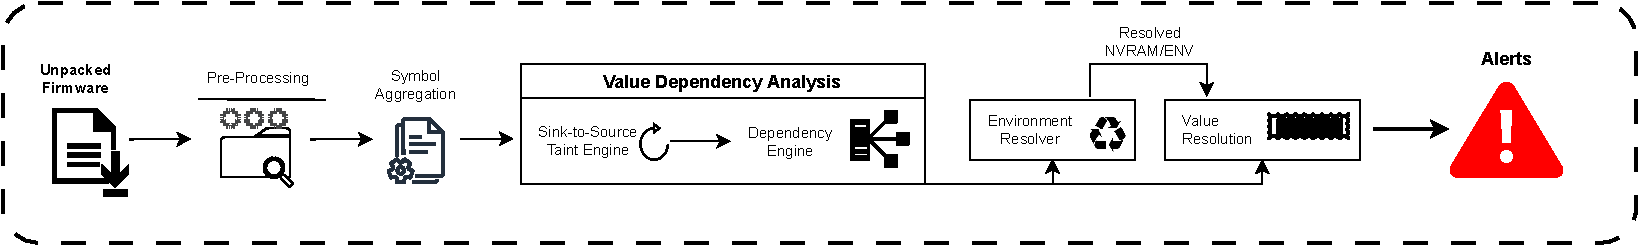
\includegraphics[width=\textwidth]{assets/diagrams/mango-flat.pdf}
    \centering
    \label{fig:mango_diagram}
    \caption{The workflow of \mango.
        \mango searches for all potential vulnerable and environment ELFs.
        It first analyzes all ELF files that can affect the environment and then analyzes all ELF files containing designated sinks with the context provided by the initial environment analysis.
    }
\end{figure*}

\mango takes a firmware image as input, analyzes all binary executables (not including library files) in the unpacked file system, and generates \trupoc{}s for potential vulnerabilities given the specified vulnerability class.
Similar to \karonte and \satc, \mango also supports multi-binary interactions and values derived from front-end keywords.
After ingesting the firmware image, \mango automatically performs subsequent analyses.
Finally, \mango outputs ranked POCs termed \trupoc{}s for the user to review.


The major analysis steps \mango performs are as follows:

\smallskip
\noindent
\textbf{Firmware Pre-processing.}
\label{sec:preprocessing}
The main goal of \mango is to analyze ELF executables and identify potential vulnerabilities.
It is important to note that we specifically do not analyze libraries as their vulnerabilities are more difficult to definitively categorize as true positives or false positives in a given firmware.
\mango takes a firmware image as input, uses existing tools (such as binwalk~\cite{binwalk}) to unpack the firmware sample, and finds all ELF executables.
For all binaries, we gather their imported library function names.
As long as the binary is not stripped and statically linked, we can recover function names such as \texttt{system} or \texttt{strcpy}.
Later, we will use these symbols to determine whether or not to analyze a given binary.


%% \smallskip
%% \noindent
%% \textbf{Filtering Vulnerable Sinks.}
%% There exist several cases in which sink callsites that are identified as vulnerable are not exploitable.
%% Some sink callsites that appear vulnerable seem to have no apparent viable path from the program start to the sink location.
%% This is most likely caused by dead code persisting across several different firmware versions or function pointers that are never actually called as part of a larger object.
%% \todo[inline]{Though it may result in false negatives, filtering such cases will greatly reduce the amount of false positives generated.}

%% Another cause of significant false positives are binaries whose intended functionality is to execute arbitrary commands.
%% \texttt{Busybox}, \texttt{tar}, \texttt{zip} as well as several other standard Linux utilities have these features.
%% As such, filtering standard tools will also reduce the false positive rate of \trupoc{}s.
%% Finally, \mango filters the results of the resolved sink values and outputs the filtered results.

\smallskip
\noindent
\textbf{Keyword Discovery.}
\satc introduced keyword-guided analysis, which increases the attack surface user input can reach and reduces the number of binaries that need to be analyzed.
\mango also gathers front-end keywords from HTML, JS, ASP, and PHP files.
These keywords are a combination of string-literals and object fields that identify user input locations in backend binaries.

\smallskip
\noindent
\textbf{IPC Discovery.}
\mango uses Inter-Process Communication (IPC) data-flow tracking, first proposed by \karonte, to detect potential interactions between binaries in a given firmware sample.
Specifically, \mango considers inter-process interactions that involve NVRAM entries and environment variables.
\mango performs static analysis (based on \rda) to collect all NVRAM and environment variables that each binary either sets or retrieves.
\mango transforms these accesses into a dictionary of setters and getters keyed by the function and recovered value (if applicable) along with which binary the value originated from and its callsite within the binary.
% The same type of analysis as the following \textit{RDA Based Data-flow Analysis} is used, except instead of finding undefined values, we are exclusively looking for defined values.

\smallskip
\noindent
\textbf{Resolving Vulnerability Sinks.}
Resolving vulnerability sinks is the core step of \mango, where, for each vulnerability sink (e.g., the glibc \texttt{system} function) in each binary, it recursively resolves the sink to a \emph{\richexpr}, which captures the source values and all operations (e.g., \texttt{strcpy} and \texttt{sprintf} with format strings) applied to these source values.
% Given any binary in the firmware, if it contains a targeted sink, we work backwards from the sink callsite finding all potential sources of input.
The sink-resolving procedure is inter-function within the same binary and inter-binary if source values originate from NVRAM entries or environment variables that \mango recovered during the IPC Discovery step.
% If we hit a known NVRAM or ENV along the way, we replace it's output with the known data.

% Library functions with defined handlers are executed to propogate their results in an effort to reduce false positives.
\mango continues sink resolving until (1) it reaches the entry point of the binary, (2) all sink values are resolved to either \emph{legitimate values} or \emph{unresolvable values}, or (3) it times out.
Legitimate values are not attacker-controllable or exploitable, such as constant values, constant pointers, or sanitized user input.
All other values are unresolvable, including user or external input and buffers with unresolvable content due to missed or unsupported library calls.




% \begin{itemize}[noitemsep]
%     \item Firmware Pre-processing (Get all symbols from elfs in firmware)
%     \item IPC discovery (Run ENV\_RESOLVE on all binaries to discover NVRAM and ENV variables)
%     \item Generate Call Traces for sink functions
%     \item Run RDA
%     \item Resolve values with SimProc Handlers
%     \item Attempt to resolve arguments at Sink Locations
%     \item Repeat steps 3-6, increasing the call-depth from the sink until max depth reached or all resolved
%     \item After all traces are resolved, filter traces and print/save results
% 
%     % Design Choices %
%     \item Assumed Execution (Expand on criteria for skipping/analyzing functions)
%     \item Bypassing Guarded loads/stores
%     \item Ignoring TOP valued pointers in sinks
% \end{itemize}

